\documentclass[13pt,oneside]{book}
\usepackage[utf8]{inputenc}
\usepackage{url}
\usepackage{graphicx}

\usepackage{geometry}
\geometry{a4paper, left=20mm, right=20mm, top=20mm, bottom=20mm}
\usepackage[margin=1.2in]{geometry}
\usepackage[toc,page]{appendix}
\usepackage{graphicx}
\usepackage{natbib}
\usepackage{lipsum}
\usepackage{caption}

\begin{document}

\captionsetup[figure]{margin=1.5cm,font=small,labelfont={bf},name={Figure},labelsep=colon,textfont={it}}
\captionsetup[table]{margin=1.5cm,font=small,labelfont={bf},name={Table},labelsep=colon,textfont={it}}
\setlipsumdefault{1}

\begin{titlepage}
\begin{center}
{\LARGE College Of Engineering Trivandrum}\\[3cm]
\linespread{1.2}\huge {\bfseries Application Software Development Lab}\\[3cm]
\linespread{1}

\includegraphics[width=5cm]{img/emblem.jpeg}\\[3cm]
{\Large GOKUL K\\ S5  CSE \\ Roll No:21\\ TVE18CS021 }\\[1cm]


\textit{ }\\[2cm]
Department of Computer Science\\[0.2cm]
\today
\end{center}

\end{titlepage}

\newpage

\begin{frame}{}
    \centering
    \hspace*{-0.5cm}
    $\vcenter{\hbox{
\includegraphics[width=1.5cm]{img/emblem.jpeg}}}$
    $\vcenter{\resizebox{0.95\textwidth}{!}{
        \begin{tabular}{c}
             CS333 - Application Software Development Lab $\cdot$ 2020 $\cdot$   \\
             \hline 
        \end{tabular}
    }}$
\end{frame}
\section*{Cycle 1}
\section*{Expt 4}
\begin{center}
    \Large{Introduction to Aggregate functions}
\end{center}

\section*{Aim}
\large{Introduction to Aggregate functions
\begin{enumerate}
	\item AVG
	\item MIN
	\item MAX
	\item SUM
	\item COUNT
\end{enumerate}
}

\section*{Experiment}
	\begin{enumerate}
		\item
		Create a table named Student and populate the table. 
				a. The table contains the marks of 10 students for 3 subjects(Physics, Chemistry, 
		 Mathematics). 
				b. The total marks for physics and chemistry is 25, while for mathematics it is 50. 
				c. The pass mark for physics and chemistry is 12 and for mathematics it is 25. 
				d. A student is awarded a ‘Pass’ if he has passed all the subjects.
		\begin{verbatim}
			+----------+----------+---------+-----------+-------------+
			| roll_num | name     | physics | chemistry | mathematics |
			+----------+----------+---------+-----------+-------------+
			|        1 | Adam     |      20 |        20 |          33 |
			|        2 | Bob      |      18 |         9 |          41 |
			|        3 | Bright   |      22 |         7 |          31 |
			|        4 | Duke     |      13 |        21 |          20 |
			|        5 | Elvin    |      14 |        22 |          23 |
			|        6 | Fetcher  |       2 |        10 |          48 |
			|        7 | Georgina |      22 |        12 |          22 |
			|        8 | Mary     |      24 |        14 |          31 |
			|        9 | Tom      |      19 |        15 |          24 |
			|       10 | Zack     |       8 |        20 |          36 |
			+----------+----------+---------+-----------+-------------+
		\end{verbatim}} 
		 
		Syntax:
		\begin{verbatim}
		CREATE TABLE IF NOT EXISTS Student (
				roll_num INT PRIMARY KEY,
				name VARCHAR(10),
				physics INT,
				chemistry INT,
				mathematics INT
		);
		INSERT INTO Student 
		VALUES
				(1, "Adam", 20, 20, 33), 
				(2, "Bob", 18, 9, 41), 
				(3, "Bright", 22, 7, 31),
				(4, "Duke", 13, 21, 20),
				(5, "Elvin", 14, 22, 23),
				(6, "Fetcher", 2, 10, 48),
				(7, "Georgina", 22, 12, 22), 
				(8, "Mary", 24, 14, 31),
				(9, "Tom", 19, 15, 24),
				(10, "Zack", 8, 20, 36);
		SELECT * FROM Student;
		
		\end{verbatim}
		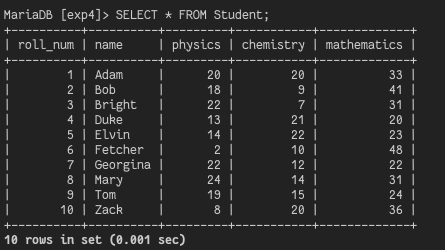
\includegraphics[]{img/p4/ss1.png}
		
		
		\item
		Find the class average for the subject ‘Physics’ 
		 
		Syntax:
		\begin{verbatim}
		SELECT AVG(physics)
		FROM Student;
		
		\end{verbatim}
		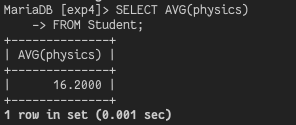
\includegraphics[]{img/p4/ss2.png}
		
		
		\item
		Find the highest marks for mathematics (To be displayed as highest\_marks\_maths). 
		 
		Syntax:
		\begin{verbatim}
		SELECT MAX(mathematics) as 'highest_marks_maths'
		FROM Student;
		
		\end{verbatim}
		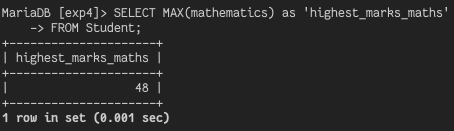
\includegraphics[]{img/p4/ss3.png}
		
		
		\item
		Find the lowest marks for chemistry(To be displayed as lowest\_mark\_chemistry) 
		 
		Syntax:
		\begin{verbatim}
		SELECT MIN(chemistry) as 'lowest_mark_chemistry'
		FROM Student;
		
		\end{verbatim}
		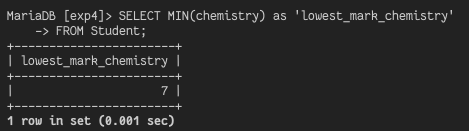
\includegraphics[]{img/p4/ss4.png}
		
		
		\item
		Find the total number of students who has got a pass in physics
		 
		Syntax:
		\begin{verbatim}
		SELECT COUNT(*)
		FROM Student
		WHERE physics >= 12;
		
		\end{verbatim}
		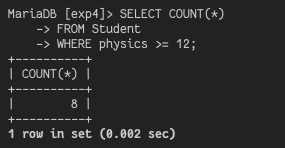
\includegraphics[]{img/p4/ss5.png}
		
		
		\item
		Generate the list of students who have passed in all the subjects. 
		 
		Syntax:
		\begin{verbatim}
		SELECT *
		FROM Student
		WHERE physics >= 12 AND chemistry >= 12 AND mathematics >= 25;
		
		\end{verbatim}
		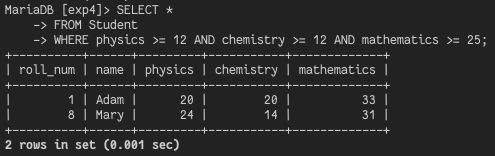
\includegraphics[]{img/p4/ss6.png}
		
		
		\item
		Generate a rank list for the class. Indicate Pass/Fail. 
		 
		Syntax:
		\begin{verbatim}
		ALTER TABLE Student
		ADD COLUMN Status VARCHAR(4) DEFAULT 'Fail';
		UPDATE Student
		SET Status='Pass'
		WHERE physics >= 12 AND chemistry >= 12 AND mathematics >= 25;
		SELECT *
		FROM Student
		ORDER BY (physics+chemistry+mathematics);
		
		\end{verbatim}
		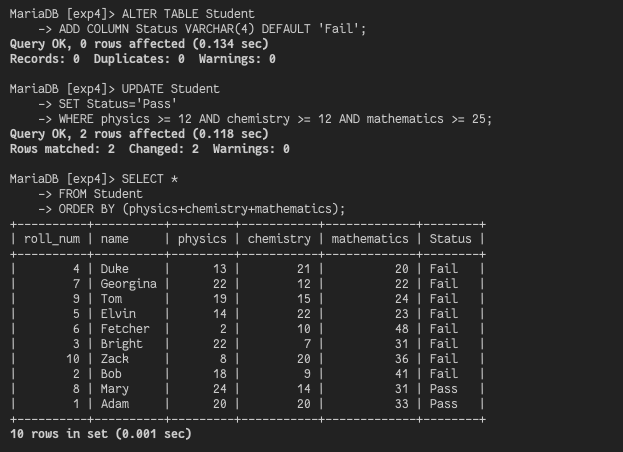
\includegraphics[]{img/p4/ss7.png}
		
		
		\item
		Find pass percentage of the class for mathematics. 
		 
		Syntax:
		\begin{verbatim}
		SELECT 100*COUNT(*)/(SELECT COUNT(*) FROM Student) as 'math_pass_percentage'
		FROM Student
		WHERE mathematics >= 25;
		
		\end{verbatim}
		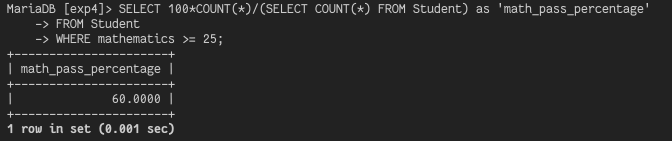
\includegraphics[]{img/p4/ss8.png}
		
		
		\item
		Find the overall pass percentage for all class. 
		 
		Syntax:
		\begin{verbatim}
		SELECT 100*COUNT(*)/(SELECT COUNT(*) FROM Student) as 'pass_percentage'
		FROM Student
		WHERE Status='Pass';
		
		\end{verbatim}
		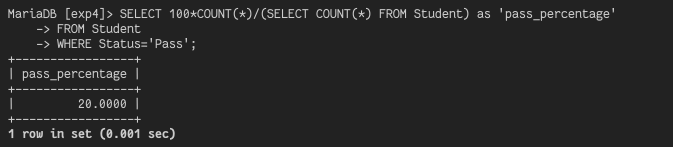
\includegraphics[]{img/p4/ss9.png}
		
		
		\item
		Find the class average. 
		 
		Syntax:
		\begin{verbatim}
		SELECT AVG(physics+chemistry+mathematics)
		FROM Student;
		
		\end{verbatim}
		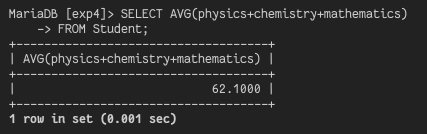
\includegraphics[]{img/p4/ss10.png}
		
		
		\item
		Find the total number of students who have got a Pass.
		
		Syntax:
		\begin{verbatim}
		SELECT COUNT(*) as 'passed'
		FROM Student
		WHERE Status='Pass';
		\end{verbatim}
		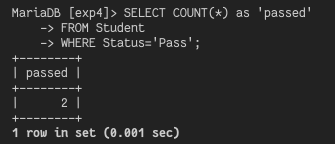
\includegraphics[]{img/p4/ss11.png}
	\end{enumerate}		
	\section*{Result}
	The basic SQL for creating and modifying a table is executed and their output
	is verified in a MySQL environment.
\end{document}